% LaTeX/AMS-LaTeX

\RequirePackage{fix-cm}
%
%\documentclass{svjour3}                     % onecolumn (standard format)
%\documentclass[smallcondensed]{svjour3}     % onecolumn (ditto)
%\documentclass[smallextended]{svjour3}       % onecolumn (second format)
\documentclass[twocolumn]{svjour3}          % twocolumn

%\documentclass{article}

\usepackage{amssymb}
\usepackage{amsmath}
%\usepackage[dvips]{graphicx}
\usepackage{graphicx}
%\usepackage{subcaption}
\usepackage{algorithm}
\usepackage{algorithmic}
\usepackage{cite}
%%%%%%%%%% NEW COMMANDS
\newcommand{\vect}[1]{\boldsymbol{#1}}

%%%%%%%%%% 
\begin{document}

\title{Studying the performance and accuracy of PFEM-2 in the solution of biomedical benchmarks}
\author{Facundo Del Pin\and Chien-Jung Huang \\ I\~naki \c{C}aldichoury\and Rodrigo R. Paz}
\institute{Livermore Software Technology Corporation\\ Livermore,  CA, United
States\\
\email{fdelpin@lstc.com}\\
\email{cjhuang@lstc.com}\\
\email{inaki@lstc.com}\\
\email{rpaz@lstc.com}}
\date{\today}

\maketitle

\begin{abstract}
In recent years the biomedical industry has shown increased interest in using numerical methods to assist in the R\&D of medical devices. The long term goal is to reduce the costly and lengthy process that clinical trials take to for the Food and Drug Administration (FDA) to approve a device. For this both FDA and academia are working together to creat laboratory experiment that will help the industry gain confidence in numerical techniques as well as provide software developers with insights on the deficiencies that numerical softeware may have. In this article three bechmarks proposed by the FDA are used to compare experimental results with those of the Finite element method (FEM) and Particle Finite Element Method 2 (PFEM-2). The first benchmark problem is the flow in a nozzle
containing a gradual and sudden change of the diameter. Several flow regimes are studied. The second problem studies the flow in a simplified centrifugal
blood pump under various pump operation conditions. Finally the third benchamrk studies the steady flow in a patient-averaged inferior vena cava. PFEM-2 is regarded as tool with great potential mainly because no stabilization is needed for the Galerkin approximation of the advection term in the transport equations. This could be a big advantage in problems with large gradients as it is the case for flows at high Reynolds number. This paper is an effort to test PFEM-2 in real world engineering applications.

\keywords{Particle Method \and Finite Element \and Biomedical Devices \and CFD \and Benchmarks \and FDA}
\end{abstract}


\section{Introduction}
A key step in the development of medical devices is the testing phase. Regulatory agencies like the Food and Drug Administration (FDA) requiere extensive laboratory testing and a long, tedioues and expensive clinical trial process before a device is approved for clinical use. In an effort to optimize this process the industry and the regulatory agencies are looking at numerical methods as an additional tool that could potentially reduce the time of product development, animal testing and cost. A first critical step to do this end is to increase the confidence, reliability and robustnece of numerical techniques. The FDA is actively working on this subject by designing laboratory experiments that could be used to evaluate the solution accuracy provided by computational methods launching the Critical Path Initiative (CPI) \cite{cpi} program. The aim of the program is to standardize the use of computational simulation on the design of the blood-contacting medical
devices and analysis of the ratio of hemolysis in them. The goal of this project is to establish the guidelines for
applying CFD on the evaluation and the optimization of the medical devices. FDA has proposed two benchmark
problems \cite{cpi1} for CFD verification and validation. The first benchmark problem is the flow in a nozzle
containing a gradual and sudden change of the diameter. The nozzle flows with different flowrates, which
correspond to different flow regimes, are examined. The second study is the flow in a simplified centrifugal
blood pump. The flow field under various pump operation conditions are analyzed. For each benchmark
problem, the experimental results \cite{fda_res},\cite{fda_nozzle}, \cite{fda_pump} and the flow field predicted with numerical simulations \cite{fda_numrob},\cite{hariharan_nozzle},\cite{nassau_pump},\cite{heck_hemo} from
different institutes are collected. The comparison between results obtained using different numerical models are
made and analyzed \cite{stewart_cfd},\cite{mali_cfd}. 

Additionally a third benchmark problem will be presented which involves the analysis of steady flow in a patient-averaged inferior vena cava \cite{gallagher_exp}, \cite{craven_cfd}. Althgouhg there are many numerical results in this area only a few compare with flow measurments of experimental results. In particular the study represents an anatomical model of the  inferior vena cava (IVC) that includes the primary morphological features that influence the hemodynamics (iliac veins, infrarenal curvature, and non-circular vessel cross-section).


In this study, these three benchmark problems will be presented and contrasted with numerical results using the Finite Element Method (FEM) and Particle Finite Element Method 2 (PFEM-2).


The main goal of this paper is to evaluate the performance of the PFEM2 method in the field of biomedical devices compareing the predictions with the experimental results. The PFEM2 method is based on the idea that advection effects are approximated in a Lagrangian way using particles. Many numerical methods are based on these ideas \cite{sph,mps,pic,mac} including the early version of PFEM \cite{sergio:PFEM}. In the latter the advection and all derivatives were computed on a finite element mesh that had to be re-constructed at every time step due to the Lagrangian nature of the method. All the fields were approximated using the FEM. The PFEM provides excellent results in problems with free surface or fluid structure interaction but it had poor performance in problems involving internal/external aerodynamics when compared to Eulerian methods due to the additional mesh operations which in turn also force a complete re-factorization of all linear systems. The work of Idelsohn et. al. \cite{sergio:xivs1,sergio:xivs2} introduced a new integration strategy called X-IVS that employed a fixed mesh modifying the PFEM and createing PFEM-2. Not only these improvements made PFEM-2 competitive in problems classically solved using Eulerian methods but it provided the advantage that larger time steps could be used \cite{gimenez:parallel} reducing the computational time in advection dominated problems and elimintating the traditional advection stabilization terms known to introduce additional numerical diffusion. By eliminating the advection term a fractional step method provides a fully decoupled momentum equation among the three velocity components which saves storage and simplify the implementation. The left hand side also becomes symetric allowing the use of simpler linear algebra solvers like Conjugate Gradient \cite{conjgrad}. The method has also been succesfully implemented for multi-phase flows \cite{sergio:pfem2_lts,gimenez:fs,gimenez:tesis}, problems invloving surface tension \cite{gimenez:st} and fluid structure interaction \cite{pablo:FSI}.

There are many applications in the biomedical field that could benefit from the capabilities of PFEM-2. In particular those applications that involve long real time simulations like drug delivery where a fluid component is injected in another fluid. In this case it is also important to keep track of the sharpt interface at the drug advancing front. {MORE APPLICATIONS}

In this work the implementation of PFEM-2 was performed in the commercial software LS-DYNA\textsuperscript{\textregistered} which is a multi-physics solver for non-linear dynamics. The module used for the implementation was ICFD which deals with incompressible fluid flows. 

The rest of this paper will be organized as follows. 
In the first section the equations governing the flow of incompressible fluids will be prsented together with boundary and initial conditions. 
In section two the PFEM-2 method will be introduced and some implementation aspects will be discussed.
In section three the time and space discretization of the equations of motion will be presented. 
In section four the benchmark problems will be introduced and the experimental and numerical results will be presented.


\section{Equations of Motion}
The benchmarks presented in this article study the motion of incompressible flows and their interaction with rigid solid boundaries. In this case the equations of motion for the continuous model are defined by the Navier-Stokes equations and the continuity equation. Let $\Omega\subset \Re^n$ be the spatial domain at time $t\in[0,T]$ with $n$ the number of space dimensions then the system of equations is defined by:
%
\begin{eqnarray}
%&\rho(\partial_t\vect{u}+\vect{u} \cdot \vect{\nabla}\vect{u})-\vect{\nabla}\cdot\sigma=\vect{f} \,\,\, \text{in}\, \Omega\times[0,T] \label{eq:mom}\\
&\rho D_t\vect{u}-\vect{\nabla}\cdot\sigma=\vect{f} \,\,\, \text{in}\, \Omega\times[0,T] \label{eq:mom}\\
&\vect{\nabla}\cdot \vect{u}=0 \label{eq:cont} \,\,\, \text{in}\, \Omega\times[0,T] 
\end{eqnarray}
%
where $\rho$ is the fluid density and $\vect{u}$ is the velocity, $\vect{f}$ is the body force and $\vect{\sigma}$ is the stress tensor:
%
\begin{equation}
\vect{\sigma}=2\mu\vect{\epsilon}(\vect{u})-p\vect{I}
\end{equation}
%
with $p$ the fluid pressure, $\mu$ the dynamic viscosity and $\vect{I}$ the identity tensor and $\vect{\epsilon}$ the strain-rate tensor defined as:
%
\begin{equation}
  \vect{\epsilon}(\vect{u})=\frac{1}{2}(\vect{\nabla}\vect{u}+\vect{\nabla}\vect{u}^t)
\end{equation}
%
Eq. (\ref{eq:mom}) needs Dirichlet and Neuman boundary conditions expressed as:
%
\begin{eqnarray}
  &\vect{u}=\vect{g} \,\,\, \text{on}\, \Gamma_g\times[0,T]\\   
  &\vect{n}\cdot\vect{\sigma}=\vect{h} \,\,\, \text{on}\, \Gamma_h\times[0,T]
\end{eqnarray}
%
where $\Gamma_g$ and $\Gamma_h$ are complementary subsets of the domain boundary $\Gamma$. The functions $\vect{g}$ and $\vect{h}$ are both given and $\vect{n}$ is the unit normal vector pointing outward from the domain.
The initial condition is specified on the domain $\Omega$ at $t=0$:
%
\begin{equation}
  \vect{u}(\vect{x},0)=\vect{u}_0(\vect{x})
\end{equation}
%
where $\vect{u}_0(\vect{x})$ is a divergence free velocity field.

The expression of Eq. (\ref{eq:mom}) was written using a material derivative since this paper will deal with both a Lagrangian and a Eulerian formulation. In the case of an Eulerian framework the material derivative becomes:
\begin{equation}
D_t\vect{u}=\partial_t\vect{u}+\vect{u} \cdot \vect{\nabla}\vect{u}  
\end{equation}
It is important to note that the last term on the right hand side is non-linear with respect to the fluid velocity $\vect{u}$.


\section{Numerical Method}
  The numerical scheme used in the approximation of the system of Eq. (\ref{eq:mom}-\ref{eq:cont}) is based on the FEM. The Galerkin method will be used with a $p1-p1$ interpolation space for the pressure-velocity pair. Furthermore the discrete model will be decoupled by means of a fractional step method as in \cite{codina-soto}. To simplify the presentation a backward difference time integration scheme was used for the time derivative of $\vect{u}$. 

\begin{align}\label{eq:masamat}
\rho \textbf{M}\vect{u}^\star+\Delta 
t\mu\textbf{K}\vect{u}^{\star} +\rho\textbf{S}(\bar{\vect{u}}^{n+1})\vect{u}^{\star}  &=\rho \textbf{M}\vect{u}^n- \Delta 
t\textbf{G}p^n+\Delta t \textbf{F},
\\\label{eq:matpres2}
\frac{\Delta t}{\rho} \textbf{L}p^{n+1}&=\textbf{D}\vect{u}^\star+ \frac{\Delta 
t}{\rho}\textbf{L}  p^{n}-\tilde{\textbf{U}},
\\\label{eq:matunm2}
\rho \bar{\textbf{M}}\vect{u}^{n+1}&=\rho \bar{\textbf{M}}\vect{u}^\star-\Delta t\textbf{G}(p^{n+1}- p^n),
\end{align}

 \subsection{The PFEM-2 method}
  The PFEM-2 method...

 \subsection{Parallel Implementation}
  The parallel implementation for PFEM-2 follows the guidelines presnted in \cite{gimenez:parallel} for the case of distributed memory architectures. The challenges are well described in their paper but basically involves the extra amount of memory needed for the particle data structure. Due to the explicit scheme the parallel implementation needs to take care of local operations to each particle separately from the rest allowing for trivial parallelization. The dificulty arise at the interface between processors where particles may travel several elements and possible processors before finding their final host element. This task requieres an outer loop to communicate particles that will terminate when no more particles cross the interface between partitions.

The current approach is built ``on top'' of a pre-existing parallel FEM implementation thus inheriting much of the data structures and methodologies. The partitions are creating using the software METIS \cite{metis}...

[Load Balancing]



[IMAGE WITH PARTICLES MOVING THROUGH PARTITIONS]



[IMAGE SCALABILITY]


 


\section{Numerical results}
% intro 
The simulations of blood flows in nozzle, pump, and IVC with FEM and PFEM-2 are conducted and compared with experimental results in \cite{fda_res}, \cite{fda_nozzle}, \cite{fda_pump} and \cite{gallagher_exp}. The fluid is assumed to be Newtonian blood analog fluid. For the nozzle and pump flows, the fluid density and viscosity are $\rho= 1035$ kg/m\textsuperscript{3} and $\mu =3.5\times10^{-3}$ N-s/m\textsuperscript{2}, where as for the flow in IVC, the density and viscosity are $\rho=1817$ kg/m\textsuperscript{3}, $\mu=5.83\times10^{-3}$ N-s/m\textsuperscript{2} for resting condition and $\mu=5.49\times10^{-3}$ N-s/m\textsuperscript{2} for exercising condition. 

\subsection{Blood Nozzle}

%  nozzle intro
The simplified nozzle proposed by FDA consists of four parts containing characteristics of some blood-conveying medical devices. There are inlet and outlet tubes with diameter $0.012$ m, as well as a cone-shaped converging tube connecting the inlet tube with the nozzle throat with diameter $0.004$ m as shown in figure~\ref{fig:nozzlegeo1}. The flow experiences a gradual contraction of area from the inlet tube to the throat, then a sudden expansion of the area right after the throat to the outlet tube (figure~\ref{fig:nozzlegeo2}). It is set that the z cordinate along the axial direction has origin at the exit of the nozzle throat. The flow with Reynolds number $3500$ with flowrate $3.64\times10^{-5}$ m\textsuperscript{3}/s corresponding to turbulent flow regime is analyzed, where the Reynolds number is defined with the flow rate and the diameter at the throat. 

%% PEGGY: should these geometry figures be included?
\begin{figure}[htbp]
    \centering
    \includegraphics[width=3.2in]{imgs/nozzle_pump/nozzle_geo.jpg}
    \caption{The dimension of the idealized nozzle model proposed by FDA.}
    \label{fig:nozzlegeo1}
\end{figure}
\begin{figure}[htbp]
    \centering
    \includegraphics[width=3.2in]{imgs/nozzle_pump/nozzle_CS.jpg}
    \caption{The flow direction and the definition of the axial coordinate z.}
    \label{fig:nozzlegeo2}
\end{figure}

%  nozzle simulation setup
For the set up of the numericcal simlation, the simulation domain starts from $z=-0.18$ m to $z=0.18$ m. The prescribed uniformly distributed velocity profile is imposed at the inlet while the pressure is constant at outlet. The turbulent flow models include the Reynolds-averaged Navier–Stokes (RANS) k-$\omega$ model and Large Eddy Simulation (LES) model are chosen to deal with the the turbulent flow regime in nozzle. The turbulence intensity is set to be $5$\% at the inlet. 

[With the LES Smagorinsky model, the Smagorinsky coefficient is set to be 0.1 empirically for flows in the pipe. Around $1.13$ million elements are used in both cases, with minimum mesh size $2.5\times10^{-4}$ m in the throat and maximum mesh size $1.0\times10^{-3}$ m in the inlet and outlet tube. As to the k-$\omega$ standard model, the domain is decomposed into about 8.61 million elements, with minimum mesh size $2.5\times10^{-4}$ m in the throat, and maximum mesh size $3.0\times10^{-4}$ m in the outlet tube.]  

% nozzle result
[Result]

% nozzle analysis
[Comparison]

\subsection{Blood Pump}

%  pump intro
The geometry of the simplified centrifugal pump is shown in the figure~\ref{fig:pumpgeo} (top). The flow enters the chamber through a curved tube with diameter $12$ mm. The diameter of the inner chamber of the housing is $60$ mm and the thickness is $9$ mm. The rotor inside the chamber is with diameter $52$ mm and $4$ mm thick, along with four $3$ mm thick straight blades. The chamber is connected with a throat at its outlet, followed by a diffuser to the outlet tube with diameter $12$ mm. The pump flow with flowrate $Q = 6$ L/min and rotational speed $3500$ RPM is simulated. 

%% PEGGY: should these geometry figures be included?
\begin{figure}[htbp]
    \centering
    \begin{minipage}[c][2.5in][c]{0.9\linewidth}
        \centering
        \includegraphics[width=3.2in]{imgs/nozzle_pump/housing_and_rotor.png}
    \end{minipage}
    \begin{minipage}[c][2.5in][c]{0.9\linewidth}
        \centering
        \includegraphics[width=3.2in]{imgs/nozzle_pump/inlet_velcocity_profile_location.png}
    \end{minipage}
    \caption{The geometry of and the flow direction in the blood pump (top), and the location where the velocity is measured in the experiments the velocity profile is prescribed in the simulations (right).}
    \label{fig:pumpgeo}
\end{figure}

%  pump simulation setup
As to the simulation set up, the velocity distribution is prescribed at the inlet (see figure~\ref{fig:pumpgeo} bottom plot), where the velocity profiles are obtained from the experimental measurements using PIV from \cite{cpi}. The pressure at the outlet is set to be constant, and the gravitational force is included. Since the goal is to predict the flow field after it reaching steady state, instead of letting the rotor rotate during simulation, the non-inertial reference frame is applied on the fluid around the rotor. This is because the flow around the rotor at steady state can be analogue to flow experiencing constant angular velocity. Using non-inertial reference frame avoids mesh distortion and frequent remeshing due to rotation. For turbulence model, the LES Smagorinsky sub-grid scale model is employed, with 7\% of turbulence intensity imposed at the inlet. 

[The simulation domain is decomposed into around 1 million tetrahedron elements as shown in figure ?.] 

% pump result
[Result]

% pump analysis
[Comparison]
\subsection{Inferior Vena Cava}

% intro
In this study, the geometry of the IVC system consists of two iliac veins merging to one infrarenal IVC as shown in figure~\ref{fig:IVCgeo}. This patient-averaged IVC geometry is proposed by \cite{gallagher_exp} from the CT data of 10 patients. The flows enter from the two iliac veins and merge after entering the infrarenal IVC, which has hydraulic diameter about $28$ mm. 
The simulations of the flow in IVC are conducted according to the parameters provided in \cite{craven_cfd}. The simulations of two flowrates are performed corresponding to the resting and exercising conditions, which are $Q= 0.5$ (l/min) and $3$ (l/min) into two iliac veins respectively. The corresponding Reynolds numbers for resting and exercising conditions are $236$ and $1505$. The flow is considered to be laminar in the IVC. For boundary conditions, the parabolic velocity profile is prescribed at the inlet of two iliac veins, and the constant pressure is imposed at the outlet of the infrarenal IVC.
In the following section, a grid convergence study is performed on the IVC flow first using FEM at the exercising condition. Secondly, the simulation results using FEM and PFEM-2 will be compared with the PIV experimental results by \cite{gallagher_exp}. 

\begin{figure}[htbp]
    \centering
    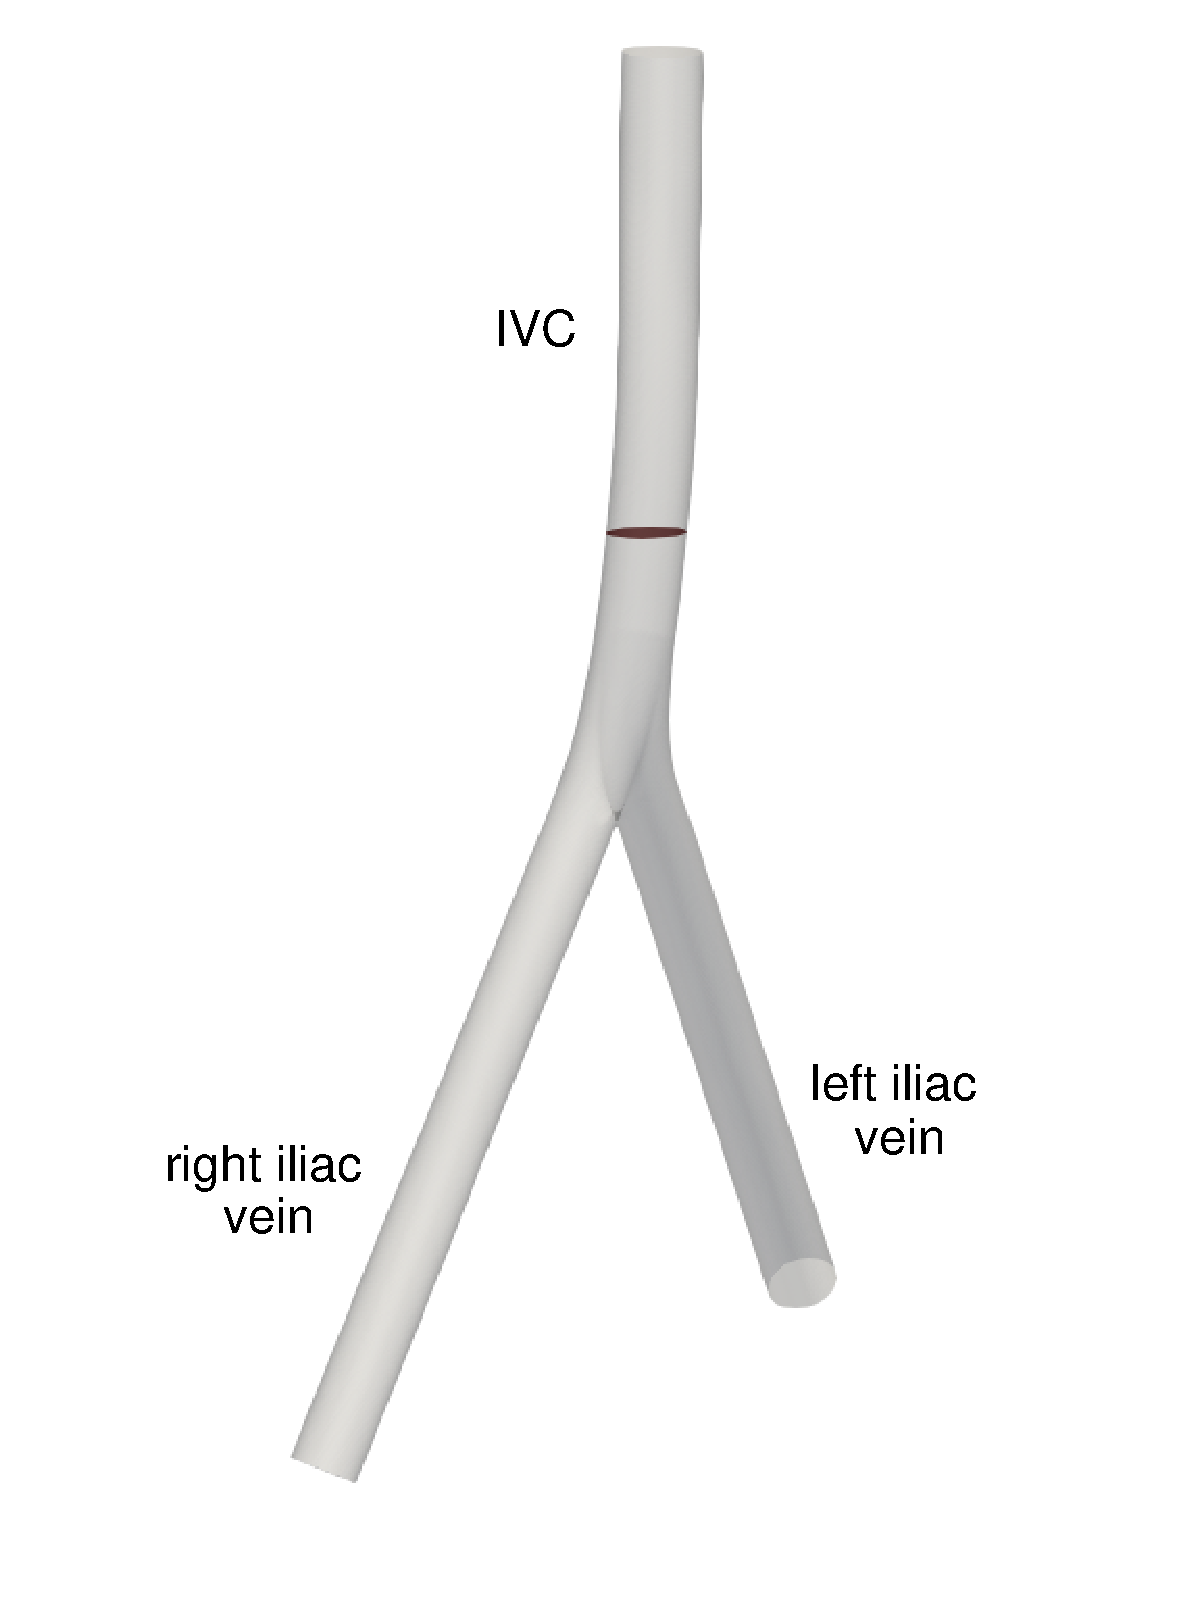
\includegraphics[scale=0.3]{imgs/vena_cava/venacava_plot.eps}
    \caption{The patient-averagved IVC geometry proposed by \cite{gallagher_exp} .}
    \label{fig:IVCgeo}
\end{figure}

\subsubsection*{Grid Convergence Test}

In the grid convergence test, five kinds of tetrahedral mesh with different mesh sizes are used. The mesh sizes are from $0.45$ mm to $2$ mm so that the domain is decomposed into to around $0.87$ million to $37.94$ million tetrahedra elements (table~\ref{tab:meshsize}). The transverse cross-sections of mesh $2$ and $4$ located at around $10$ cm downstream of the confluence of two iliac veins are shown in the figure~\ref{fig:IVCmesh}.

\begin{table}[h]
\caption {Mesh used in the convergence test.} \label{tab:meshsize}
\centering
\begin{tabular}{|c|c|c|}
\hline
Mesh & Number of element ($\times10^6$)& mesh size (mm) \\ \hline
1    & 0.87              & 2.0              \\ \hline
2    & 2.04              & 1.4            \\ \hline
3    & 4.70              & 1.0               \\ \hline
4    & 17.68             & 0.6            \\ \hline
5    & 37.94             & 0.45            \\ \hline
\end{tabular}
\end{table}

\begin{figure}[h]\centering
    \includegraphics[width=0.5\linewidth]{imgs/vena_cava/mesh2_fixed.png}
    \includegraphics[width=0.5\linewidth]{imgs/vena_cava/mesh4.png}
    \caption{The transverse cross-sectional view of mesh number 2 (top) and number 4 (bottom) in the grid convergence study. The cross-section is located at around 10 cm downstream of the confluence of two iliac veins.}
    \label{fig:IVCmesh}
\end{figure}

The flow simulations with these five meshes are conducted using FEM at exercising condition. The simulation result will be evaluated not only qualitatively with the velocity magnitude field and local normalized helicity field on a transverse cross-sectional plane, but also quantitatively through three scalar quantities: maximum nodal velocity, area-averaged transverse velocity magnitude and volume-averaged helicity intensity. The helicity density $h$, which is defined as the inner product of vorticity and velocity $h=u\cdot\omega$, represents the tendency of the flow to have helical flow. The local normalized helicity (LNH) is 
\begin{equation}
LNH=\frac{u\cdot\omega}{\left|u\right|\left|\omega\right|},
\label{eq:LNH}
\end{equation}
and the volume-averaged helicity intensity $\overline{HI}$ can be calculated using
\begin{equation}
\overline{HI}=\frac{1}{V}\int_V \left|u\cdot\omega\right| dV.
\label{eq:HI}
\end{equation}
The area-averaged transverse velocity magnitude,
\begin{equation}
\overline{\left|u_{tr}\right|}=\frac{1}{A}\int_A \left|u _\|\right| dA,
\label{eq:utr}
\end{equation}
where $u _\|$ is the velocity component parallel to the surface, indicates the measure of the secondary flow. The velocity magnitude field, LNH, and $\overline{\left|u_{tr}\right|}$ will be examined on the transverse cross-sectional plane located at $10$ cm downstream of the confluence point in the present study.  

The obtained velocity magnitude field and LNH field with above-mentioned five meshes on the same transverse cross-sectional plane are shown in figure \ref{fig:velmag} and \ref{fig:lnh}. It can be observed that the resulting flow velocity fields with different sizes of meshes have the similar patterns, but the some flow details are unresolved with mesh $1$ and $2$. This phenomenon can also be seen in the resulting LNH fields.

\begin{figure*}[htbp]
    \centering
    \begin{minipage}[c][2in][c]{0.4\linewidth}
        \centering
        \includegraphics[width=2.3in]{imgs/vena_cava/Umag_mesh1.png}\\
        mesh 1
    \end{minipage}
    \begin{minipage}[c][2in][c]{0.4\linewidth}
        \centering
        \includegraphics[width=2.3in]{imgs/vena_cava/Umag_mesh2.png}\\
        mesh 2
    \end{minipage}\\[.5\baselineskip]
    \begin{minipage}[c][2in][c]{0.4\linewidth}
        \centering
        \includegraphics[width=2.3in]{imgs/vena_cava/Umag_mesh3.png}\\
        mesh 3
    \end{minipage}
    \begin{minipage}[c][2in][c]{0.4\linewidth}
        \centering
        \includegraphics[width=2.3in]{imgs/vena_cava/Umag_mesh4.png}\\
        mesh 4
    \end{minipage}\\[.5\baselineskip]
    \begin{minipage}[c][2in][c]{0.4\linewidth}
        \centering
        \includegraphics[width=2.3in]{imgs/vena_cava/Umag_mesh5.png}\\
        mesh 5
    \end{minipage}
    \begin{minipage}[c][2in][c]{0.4\linewidth}
        \centering
        \includegraphics[width=.7in]{imgs/vena_cava/colormap_exercise.png}\\
    \end{minipage}
    \caption{The velocity magnitude fields using different sizes of mesh.}
    \label{fig:velmag}
\end{figure*}

\begin{figure*}[htbp]
    \centering
    \begin{minipage}[c][2in][c]{0.4\linewidth}
        \centering
        \includegraphics[width=2.3in]{imgs/vena_cava/LNH_mesh1.png}\\
        mesh 1
    \end{minipage}
    \begin{minipage}[c][2in][c]{0.4\linewidth}
        \centering
        \includegraphics[width=2.3in]{imgs/vena_cava/LNH_mesh2_fixed.png}\\
        mesh 2
    \end{minipage}\\[.5\baselineskip]
    \begin{minipage}[c][2in][c]{0.4\linewidth}
        \centering
        \includegraphics[width=2.3in]{imgs/vena_cava/LNH_mesh3.png}\\
        mesh 3
    \end{minipage}
    \begin{minipage}[c][2in][c]{0.4\linewidth}
        \centering
        \includegraphics[width=2.3in]{imgs/vena_cava/LNH_mesh4_fixed.png}\\
        mesh 4
    \end{minipage}\\[.5\baselineskip]
    \begin{minipage}[c][2in][c]{0.4\linewidth}
        \centering
        \includegraphics[width=2.3in]{imgs/vena_cava/LNH_mesh5.png}\\
        mesh 5
    \end{minipage}
    \begin{minipage}[c][2in][c]{0.4\linewidth}
        \centering
        \includegraphics[width=.7in]{imgs/vena_cava/colormap_LNH.png}\\
    \end{minipage}
    \caption{The local normalized helicity (LNH) fields.}
    \label{fig:lnh}
\end{figure*}

The quantitative analysis of the convergence study using maximum nodal velocity, area-averaged transverse velocity magnitude and volume-averaged helicity intensity are tabulated in table~\ref{tab:convergence}, where $p$ represent the order of convergence [ADD REFERENCE].
It can be observed that the transverse velocity and helicity values converge when meshes get finer. But for the maximum nodal velocity, the trend is monotonic except for the result by mesh $1$. This might be because the nodal maximum velocity is still affected by how the domain is decomposed. In the following section, the mesh $2$ and $3$ will be utilized in the simulation of IVC flows at resting and exercising conditions.

% choose either one: with  p or not with p
\begin{table*}[]
\centering
\caption {The value of maximum velocity, transverse velocity, Helicity and the corresponding order of convergence $p$.} \label{tab:convergence}
\begin{tabular}{|c|c|c|c|c|c|c|}
\hline
     & \multicolumn{2}{c|}{maximum velocity} & \multicolumn{2}{c|}{transverse velocity} & \multicolumn{2}{c|}{Helicity} \\ \hline
Mesh & $\left |u\right |_{max} $    & p             & $\overline{\left |u_{tr}\right |}$          & p              &   $\overline{HI}$              & p           \\ \hline
1    & 0.2549               &               & 0.0238                 &                & 0.3807         &             \\ \hline
2    & 0.2585               &               & 0.0244                 &                & 0.4132         &             \\ \hline
3    & 0.2567               & 2.36       & 0.0247                 & 2.40          & 0.4331         & 1.63        \\ \hline
4    & 0.2541               & 0.31       & 0.02497                 & 2.24          & 0.4498         & 1.84        \\ \hline
5    & 0.2534	          &  2.16      & 0.02502                 & 2.88          & 0.4536         &  2.54        \\ \hline
\end{tabular}
\end{table*}
% 
\iffalse
\begin{table}[h]
\caption {} \label{tab:convergence}
\centering
\begin{tabular}{|c|c|c|c|}
\hline
Mesh & $u_{max}$ & Transverse velocity &  Helicity       \\ \hline
1    & 0.25486           & 0.02380        & 0.38067 \\ \hline
2    & 0.25846           & 0.02443        & 0.41316 \\ \hline
3    & 0.25666           & 0.02474        & 0.43313 \\ \hline
4    & 0.25409           & 0.02497        & 0.44978 \\ \hline
5     & 0.25341	      & 0.02502        & 0.45361         \\ \hline
\end{tabular}
\end{table}
\fi
%------------------------------------

\subsubsection*{Comparison with Experimental Results}

The velocity fields predicted by FEM and PFEM-2 solvers will be compared quantitatively with PIV experimental result by \cite{gallagher_exp} on a selected sagittal plane and a coronal plane indicated at two flow conditions in figure~\ref{fig:IVCPIV}. The FEM and PFEM-2 solvers use the same mesh under the same flow condition. The experimental and simulation results of the in-plane 2D velocity magnitudes in the sagittal and coronal planes at resting and exercising conditions are shown in the figure \ref{fig:rest} and \ref{fig:exercise}. It shows that the results by FEM and PFEM-2 solvers both match qualitatively with the PIV results. 

\begin{figure}[htbp]
    \centering
    \includegraphics[scale=0.3]{imgs/vena_cava/PIV_plane_rest.png}
    \caption{The sagittal and coronal planes where the velocity field are measured in experiments (\cite{gallagher_exp}) [PLOT NEEDS TO BE REDONE].}
    \label{fig:IVCPIV}
\end{figure}

\begin{figure*}\centering
\begin{minipage}[c][10cm][c]{0.25\textwidth}
\centering
\vspace*{\fill}
\includegraphics[height=4cm]{imgs/vena_cava/PIV_coronal_rest.png}
\includegraphics[height=5cm]{imgs/vena_cava/PIV_sagittal_rest.png}
\\PIV
\end{minipage}
\begin{minipage}[c][10cm][c]{0.25\textwidth}
\centering
\vspace*{\fill}
\includegraphics[height=4cm]{imgs/vena_cava/FEM_coronal_rest.png}
\includegraphics[height=5cm]{imgs/vena_cava/FEM_sagittal_rest.png}
\\FEM
\end{minipage}
\begin{minipage}[c][10cm][c]{0.25\textwidth}
\centering
\vspace*{\fill}
\includegraphics[height=4cm]{imgs/vena_cava/PFEM_coronal_rest.png}
\includegraphics[height=5cm]{imgs/vena_cava/PFEM_sagittal_rest.png}
\\PFEM-2
\end{minipage}
\begin{minipage}[c][10cm][t]{0.1\textwidth}
\vspace*{\fill}
\centering
\includegraphics[height=3cm]{imgs/vena_cava/colormap_rest.png}
\\
\end{minipage}
\caption{The in-plane 2D velocity magnitude in coronal (top) and sagittal (bottom) planes of PIV, FEM and PFEM-2 results at resting condition}
\label{fig:rest}
\end{figure*}

\begin{figure*}\centering
\begin{minipage}[c][10cm][c]{0.25\textwidth}
\centering
\vspace*{\fill}
\includegraphics[height=4cm]{imgs/vena_cava/PIV_coronal_exercise.png}
\includegraphics[height=5cm]{imgs/vena_cava/PIV_sagittal_exercise.png}
\\PIV
\end{minipage}
\begin{minipage}[c][10cm][c]{0.25\textwidth}
\centering
\vspace*{\fill}
\includegraphics[height=4cm]{imgs/vena_cava/FEM_coronal_exercise.png}
\includegraphics[height=5cm]{imgs/vena_cava/FEM_sagittal_exercise.png}
\\FEM
\end{minipage}
\begin{minipage}[c][10cm][c]{0.25\textwidth}
\centering
\vspace*{\fill}
\includegraphics[height=4cm]{imgs/vena_cava/PFEM_coronal_exercise.png}
\includegraphics[height=5cm]{imgs/vena_cava/PFEM_sagittal_exercise.png}
\\PFEM-2
\end{minipage}
\begin{minipage}[c][10cm][t]{0.1\textwidth}
\vspace*{\fill}
\centering
\includegraphics[height=3cm]{imgs/vena_cava/colormap_exercise.png}
\\
\end{minipage}
\caption{The in-plane 2D velocity magnitude in coronal (top) and sagittal (bottom) planes of PIV, FEM and PFEM-2 results at resting condition}
\label{fig:exercise}
\end{figure*}

To do quantitative comparison with experiments, the numerically obtained nodal velocities are firstly sampled on to the PIV data points. The magnitude of 2D plane velocity is then calculated on each data points. The global relative error, $E$, can be obtained by averaging the relative error between numerical and experimental result on all the points. Table \ref{tab:rest} and \ref{tab:exercise} shows the global relative error at different flow conditions with FEM, PFEM-2 solvers as well as the numerical analysis reported in \cite{craven_cfd}. The global relative error is around $5$ to $6$\% at resting condition and $6$ to $11$\% at exercising condition. The numerical results have a good agreement with the experimental data. For both conditions, the FEM and PFEM-2 results have similar amount of global relative error with \cite{craven_cfd}. It is worth noting that the mesh sizes used here ($1.4$ mm for resting and $1$ mm for exercising) are coarser than the mesh size ($0.276$ mm) used in \cite{craven_cfd}. Also, the PFEM-2 has nearly the same error with FEM at resting condition, and even less error in the coronal plane at exercising condition.

\begin{table}[h!]
\caption {Global relative error (\%) between CFD and PIV at resting condition.} \label{tab:rest}
\centering
\begin{tabular}{|c|c|c|}
\hline
       & Coronal & Sagittal \\ \hline
\cite{craven_cfd}  & 3.07    & 6.77     \\ \hline
FEM    & 4.83    & 6.62     \\ \hline
PFEM-2 & 4.79    & 6.65     \\ \hline
\end{tabular}
\end{table}

\begin{table}[h!]
\caption {Global relative error (\%) between CFD and PIV at exercising condition.} \label{tab:exercise}
\centering
\begin{tabular}{|c|c|c|}
\hline
       & Coronal & Sagittal \\ \hline
\cite{craven_cfd}  & 10.98	&5.56 \\ \hline
FEM    &  11.28    &  5.93  \\ \hline
PFEM-2 &  10.44   &  6.10     \\ \hline
\end{tabular}
\end{table}


\section{Conclusions}

%\clearpage
\begin{thebibliography}{9}
  \bibitem{cpi1} FDA’s ``Critical Path'' Computational Fluid Dynamics (CFD)/Blood Damage Project: Computational Round Robin problems
https://nciphub.org/wiki/FDA\_CFD
\bibitem{cpi} FDA Critical Path Initiative (CPI) \\\small{https://www.fda.gov/scienceresearch/specialtopics/criticalpathinitiative/default.htm}
\bibitem{fda_res} Hariharan, P., Giarra, M., Reddy, V., Day, S.W.,
Manning, K.B., Deutsch, S., Stewart, S.F., Myers, M.R., Berman, M.R., Burgreen, G.W. and Paterson, E.G. (2011).
Multilaboratory particle image velocimetry analysis of the FDA benchmark nozzle model to support validation of computational
fluid dynamics simulations. Journal of Biomechanical Engineering, 133(4), 041002.
\bibitem{fda_nozzle} Herbertson, L. H., Olia, S. E., Daly, A., Noatch, C. P., Smith, W. A., Kameneva, M. V., \& Malinauskas, R. A. (2015).
Multilaboratory Study of Flow‐Induced Hemolysis Using the FDA Benchmark Nozzle Model. Artificial organs, 39(3), 237-248.
\bibitem{fda_pump} Giarra, M. N. (2009). Shear Stress Distribution and Hemolysis Measurements in a Centrifugal Blood Pump. Rochester Institute of
Technology.
\bibitem{fda_numrob} Zmijanovic, V., Mendez, S., Moureau, V., \& Nicoud, F. (2017). About the numerical robustness of biomedical benchmark cases:
Interlaboratory FDA's idealized medical device. International journal for numerical methods in biomedical engineering, 33(1).
\bibitem{hariharan_nozzle} Hariharan, P., D’Souza, G. A., Horner, M., Morrison, T. M., Malinauskas, R. A., \& Myers, M. R. (2017). Use of the FDA nozzle
model to illustrate validation techniques in computational fluid dynamics (CFD) simulations. PloS one, 12(6), e0178749.
\bibitem{nassau_pump} Nassau, C. J., Wray, T. J., \& Agarwal, R. K. (2015, July). Computational Fluid Dynamic Analysis of a Blood Pump: An FDA
Critical Path Initiative. In ASME/JSME/KSME 2015 Joint Fluids Engineering Conference (pp. V002T26A002-V002T26A002).
American Society of Mechanical Engineers.
\bibitem{heck_hemo} Heck, M. L., Yen, A., Snyder, T. A., O'Rear, E. A., \& Papavassiliou, D. V. (2017). Flow‐Field Simulations and Hemolysis
Estimates for the Food and Drug Administration Critical Path Initiative Centrifugal Blood Pump. Artificial organs, 41(10).
\bibitem{stewart_cfd} Stewart, S. F., Paterson, E. G., Burgreen, G. W., Hariharan, P., Giarra, M., Reddy, V., Stewart, S.F., Paterson, E.G., Burgreen,
G.W., Hariharan, P., Giarra, M., Reddy, V., Day, S.W., Manning, K.B., Deutsch, S., Berman, M.R. and Myers, M.R. (2012).
Assessment of CFD performance in simulations of an idealized medical device: results of FDA’s first computational
interlaboratory study. Cardiovascular Engineering and Technology, 3(2), 139-160.
\bibitem{mali_cfd} Malinauskas, R. A., Hariharan, P., Day, S. W., Herbertson, L. H., Buesen, M., Steinseifer, U., Aycock, K.I., Good, B.C., Deutsch,
S., Manning, K.B. and Craven, B.A. (2017). FDA benchmark medical device flow models for CFD validation. ASAIO Journal,
63(2), 150-160.
\bibitem{gallagher_exp} Gallagher, M. B., Aycock, K. I., Craven, B. A., \& Manning, K. B. (2018). Steady flow in a patient-averaged inferior vena cava—part I: particle image velocimetry measurements at rest and exercise conditions. Cardiovascular engineering and technology, 9(4), 641-653.
% Gallagher, M.B., Aycock, K.I., Craven, B.A. et al. Cardiovasc Eng Tech (2018) 9: 641. https://doi.org/10.1007/s13239-018-00390-2
\bibitem{craven_cfd} Craven, B. A., Aycock, K. I.,\& Manning, K. B. (2018). Steady Flow in a Patient-Averaged Inferior Vena Cava—Part II: Computational Fluid Dynamics Verification and Validation. Cardiovascular engineering and technology, 9(4), 654-673.
%Craven, B.A., Aycock, K.I. \& Manning, K.B. Cardiovasc Eng Tech (2018) 9: 654. https://doi.org/10.1007/s13239-018-00392-0
\bibitem{sph} Monaghan JJ (1988) An introduction to SPH. Comput Phys Com-
mun 48:89–96
\bibitem{pic} Harlow FH (1955) A machine calculation method for hydro-
dynamic problems. Los Alamos Scientific Laboratory Report
LAMS-1956
\bibitem{mac} Harlow FH, Welch J (1965) Numerical calculation of time depen-
dent viscous incompressible flow of fluid with free surface. Phys
Fluids 8(12):2182–2189
\bibitem{mpm} Wieckowsky Z (2004) The material point method in large
strain engineering problems. Comput Methods Appl Mech Eng
193(39):4417–4438
\bibitem{sergio:pfem} Idelsohn SR, Oñate E, Del Pin F (2004) The particle finite element
method a powerful tool to solve incompressible flows with free-
surfaces and breaking waves. Int J Numer Methods 61:964–989

\bibitem{sergio:xivs1} Idelsohn SR, Nigro NM, Limache A, Oñate E (2012) Large
time-step explicit integration method for solving problems with
dominant convection. Comput Methods Appl Mech Eng 217–
220:168–185

\bibitem{sergio:xivs2} Idelsohn SR, Nigro NM, Gimenez JM, Rossi R, Marti J (2013)
A fast and accurate method to solve the incompressible Navier–
Stokes equations. Eng Comput 30(2):197–222

\bibitem{gimenez:parallel} Gimenez JM, Nigro NM, Idelsohn SR (2014) Evaluating the perfor-
mance of the particle finite element method in parallel architectures.
J Comput Part Mech 1(1):103–116

\bibitem{sergio:pfem2_lts} Idelsohn SR, Marti J, Becker P, Oñate E (2014) Analysis of mul-
tifluid flows with large time steps using the particle finite element
method. Int J Numer Methods Fluids 75(9):621–644

\bibitem{gimenez:fs} Gimenez JM, Gonzlez LM (2015) An extended validation of the
last generation of particle finite element method for free surface
flows. J Comput Phys 284:186–205
\bibitem{pablo:FSI} Becker P, Idelsohn SR, Oñate E (2014) A unified monolithic
approach for multi-fluid flows and fluid-structure interaction using
the particle finite element method with fixed mesh. Comput Mech
55(6):1091–1104
\bibitem{gimenez:st} Gimenez JM, Nigro N, Oñate E, Idelsohn S (2016) Surface tension
problems solved with the particle finite element method using large
time-steps. Comput Fluids
\bibitem{gimenez:tesis} Gimenez JM (2015) Enlarging time-steps for solving one and two
phase flows using the particle finite element method. Ph.D. Thesis,
Universidad Nacional del Litoral, Santa Fe, Argentina
\bibitem{codina-soto} Ramon Codina, Orlando Soto,
Approximation of the incompressible Navier–Stokes equations using orthogonal subscale stabilization and pressure segregation on anisotropic finite element meshes,
Computer Methods in Applied Mechanics and Engineering,
Volume 193, Issues 15–16,
2004,
Pages 1403-1419,
ISSN 0045-7825,
https://doi.org/10.1016/j.cma.2003.12.030.
\bibitem{codina-oss-press} Ramon Codina,
Stabilization of incompressibility and convection through orthogonal sub-scales in finite element methods,
Computer Methods in Applied Mechanics and Engineering,
Volume 190, Issues 13–14,
2000,
Pages 1579-1599,
ISSN 0045-7825,
https://doi.org/10.1016/S0045-7825(00)00254-1.
\bibitem{chorin}
A.J. Chorin, Math. Comput. 22,745 (1968)
\bibitem{temam}
R. Temam, Arch. Rat. Mech. Anal. 32, 377 (1969)
\bibitem{tesis-gimenez}  J. Gimenez, Enlarging time steps for solving one and two phase flows using the particle finite element
 method, Ph.D. thesis, Facultad de Ingenier\'{\i}a y Ciencias H\'{\i}dricas - Centro de Investigaciones en Mecanica
 Computacional. Santa Fe, Argentina (2015).

\end{thebibliography}
\end{document}
